
\begin{table}[t]
\centering
\small
\caption{Six clean-useful high-SER pairs: clean transplant remains deployable (PPL ratio $\le 1.25\times$, max accuracy drop $\le 0.02$, zero failed tasks), yet the attack still drives high attacked-base SER while keeping donor SER near zero.}
\label{tab:clean-useful}
\begin{tabular}{llrrrr}
\toprule
Base & Donor & SER$_{\max}$(base) & SER$_{\max}$(donor) & Clean Wikitext $\times$ & Max clean acc.\ drop \\
\midrule
Gem3-1B   & Gem2-2B & 1.000 & 0.000 & 1.216 & 0.012 \\
L3.2-3B   & L3.1-8B & 1.000 & 0.000 & 1.002 & 0.007 \\
L3.2-3B   & ML3-8B  & 1.000 & 0.000 & 1.002 & 0.007 \\
M7B-v0.1  & Min-3B  & 0.977 & 0.047 & 1.003 & 0.002 \\
Q2.5-1.5B & Q2-7B   & 0.926 & 0.027 & 0.999 & 0.009 \\
Q2.5-1.5B & Q3-14B  & 0.906 & 0.000 & 0.999 & 0.008 \\
\bottomrule
\end{tabular}
\end{table}

\section{Clean-useful high-SER examples on deployable composed models}
\label{app:clean_useful}

The \emph{clean-useful} filter is computed from the clean OMP transplant only: it does not consult attacked-base SER, donor SER, or any other attack-side quantity. A pair passes when its \emph{clean} OMP transplant (i) records zero failed evaluation tasks, (ii) keeps Wikitext-PPL within $1.25\times$ the original (before-OMP) base value, and (iii) keeps the maximum drop on the accuracy benchmarks within $0.02$, all relative to the original base before any OMP step. Table~\ref{tab:clean-useful} then reports the six pairs that pass this filter \emph{and additionally} reach high attacked-base SER with near-zero donor SER; the second criterion is reported for the table but is not used in the filter.
On these pairs, the composed model remains usable on standard utility benchmarks while still being susceptible to the attack: attack success is not contingent on pre-existing transplant brittleness.

\section{Baseline comparisons}
\label{app:baselines}

The asymmetric-realizability mechanism is not reproduced by generic one-token appends. We compare our designed breaker token against two appended-token baselines under the identical OMP transplant pipeline and SER protocol:
\begin{itemize}[leftmargin=*,nosep]
    \item \textbf{random}: append a single new token whose donor-side embedding is drawn isotropically and rescaled to match the median donor embedding norm.
    \item \textbf{high\_norm}: append a single new token whose donor-side embedding is sampled isotropically and then rescaled to several times the median donor norm.
\end{itemize}
Table~\ref{tab:baselines} compares these against our \emph{proposed} designer on two representative pairs.

\begin{table}[!htbp]
\centering
\small
\setlength{\tabcolsep}{3pt}
\caption{Generic one-token appends do not produce asymmetric realization. Random and high-norm appends fail to drive attacked-base SER above zero on either pair, while our designer reaches high attacked-base SER with only mild base-side utility shift.}
\label{tab:baselines}
\begin{minipage}[t]{0.49\linewidth}
  \centering
  \textbf{Q2-0.5B $\leftarrow$ Gem3-1B}\\[2pt]
  \begin{tabular}{lrrrr}
  \toprule
  Method & SER$_{\max}$(b) & SER$_{\max}$(d) & $\Delta$PPL & $\Delta$LBD \\
  \midrule
  proposed   & 0.645 & 0.078 & 1.290 & $-0.011$ \\
  random     & 0.000 & 0.000 & 0.000 & $+0.054$ \\
  high\_norm & 0.000 & 0.965 & 0.000 & $+0.054$ \\
  \bottomrule
  \end{tabular}
\end{minipage}\hfill
\begin{minipage}[t]{0.49\linewidth}
  \centering
  \textbf{Gem3-1B $\leftarrow$ Gem2-2B}\\[2pt]
  \begin{tabular}{lrrrr}
  \toprule
  Method & SER$_{\max}$(b) & SER$_{\max}$(d) & $\Delta$PPL & $\Delta$LBD \\
  \midrule
  proposed   & 1.000 & 0.000 & 14.889 & $-0.110$ \\
  random     & 0.000 & 0.000 & 0.000  & $+0.010$ \\
  high\_norm & 0.000 & 0.000 & 0.000  & $+0.010$ \\
  \bottomrule
  \end{tabular}
\end{minipage}
\end{table}

The pattern is sharp: random and high-norm one-token appends fail to drive attacked-base SER above zero on either pair, even when (in the Q2-0.5B$\leftarrow$Gem3-1B case) the high-norm baseline does leak on the donor. Our designer is the only method that produces the asymmetric realization the threat model requires: high attacked-base SER together with a near-silent donor.

\section{Cross-base transfer and multi-victim bundling}
\label{app:transfer_bundling}

Cross-base transfer and multi-victim bundling test how the construction behaves when the same donor artifact is used against bases beyond the seed pair. The first experiment transplants a donor row optimized for one base into a different base. The second patches one donor with multiple breaker rows, each targeting a different base.

\noindent\textbf{Cross-base transfer.}
Table~\ref{tab:cross-base} shows transfer from a designed seed pair to a different base. The breaker tokens transfer to held-out bases with non-trivial attacked-base SER while keeping donor SER essentially zero.

\begin{table}[!htbp]
\centering
\small
\caption{Cross-base transfer of designed breaker tokens. ``Seed base'' is the base the token was optimized against; ``Transferred base'' is a different base into which the same donor (with the same designed breaker row) is then transplanted. The attack transfers under zero-shot conditions.}
\label{tab:cross-base}
\begin{tabular}{lcccc}
\toprule
Breaker seed & Seed-base SER$_{\max}$ & Transferred base & Transferred-base SER$_{\max}$ & Donor SER$_{\max}$ \\
\midrule
Gem2-2B$\leftarrow$Q2-0.5B & 0.7734 & Min-3B  & 0.7578 & 0.0078 \\
Gem2-2B$\leftarrow$Q3-0.6B & 0.8789 & Gem3-1B & 0.3047 & 0.0000 \\
\bottomrule
\end{tabular}
\end{table}

\noindent\textbf{Multi-victim bundling.}
A single donor can also be patched with multiple breaker tokens, each optimized for a different base. Table~\ref{tab:bundling} reports a setting where one Gem2-2B donor carries 5 breakers targeting 5 different bases simultaneously. The donor's any-token SER stays at zero, and all 5 attacked bases hit bundled-token SER$_{\max}{=}1.0$, with 4 of 5 also hitting their \emph{intended} target base at SER$_{\max}\ge 0.5$.

\begin{table}[t]
\centering
\small
\caption{Multi-victim bundling: one Gem2-2B donor patched with 5 breaker tokens, each targeting a different base. Donor stealth is preserved on all five tokens, while every attacked base hits a bundled-token SER$_{\max}{=}1.0$.}
\label{tab:bundling}
\begin{tabular}{lr}
\toprule
Metric & Value \\
\midrule
Donor model                                              & Gem2-2B \\
Inserted breaker tokens in one donor                     & 5 \\
Donor any-token SER$_{\max}$                             & 0.000 \\
Attacked bases with any bundled-token SER$_{\max}{=}1.0$ & 5 / 5 \\
Attacked bases with intended-token SER$_{\max}\ge 0.5$   & 4 / 5 \\
\bottomrule
\end{tabular}
\end{table}

\noindent\textbf{Why bundling persistence is essentially implied by the pairwise result.}
By definition, any shared-basis transplant operator (OMP, CLP, WECHSEL, FOCUS) reconstructs each donor-only row as a function of the shared anchor set $\mathcal{T} = \mathcal{V}_b \cap \mathcal{V}_d$ alone, without interaction across donor-only rows. The anchor set is fixed by the donor and base vocabularies; appending additional donor-only bundle tokens leaves it unchanged. Each bundle row's recovered coefficients (and hence its base-side reconstruction) are therefore identical to those obtained when only that row is appended, regardless of the operator class. The base model's transformer parameters and LM head are likewise unchanged between the pairwise and bundled settings, so the last-layer hidden states on any fixed prompt are identical, and each individual bundle breaker receives the same per-context logit as in the pairwise case. The only new dynamic is competition between bundle breakers for the top-1 position when several of them receive high logits on the same prompt. From the attacker's perspective this is generally a feature: the attack goal is realized whenever any bundle breaker fires, so bundled-token $\mathrm{SER}_{\max}$ lower-bounds the maximum pairwise SER over the bundle, and the bundle widens the attack's effective coverage. The argument places no upper bound on bundle size: any number of donor-only rows leaves the shared anchor set unchanged, and bundled-token $\mathrm{SER}_{\max}$ is monotonically non-decreasing in the number of breakers added. Operationally, the attacker therefore pre-computes one breaker row per intended base offline and bundles all of them into a single donor checkpoint, with no per-row degradation relative to the pairwise setting. The resulting donor compromises every deployer using a base from the targeted set without any per-deployment action at runtime; the relevant practical scale is the cardinality of deployment targets the attacker chooses to cover, set by the structure of the open-weight LLM ecosystem rather than by the tokenizer's vocabulary capacity.

\noindent\textbf{Implications for the supply-chain story.}
Together, these results substantiate the supply-chain framing under realistic open-weight conditions. Cross-base transfer shows zero-shot activation in held-out bases with the donor remaining silent. Multi-victim bundling shows that a single donor artifact can carry several base-specific breaker rows at once with no per-row cost relative to the pairwise setting.

\section{Cross-domain failure of LoRA fine-tuning}
\label{app:lora_persistence}

\noindent\textbf{Setup.}
We fine-tune LoRA defenders on the post-transplant attacked base for two pairs at $\lambda{=}2048$: Q2-0.5B$\leftarrow$Min-3B (the primary case study) and Q3-0.6B$\leftarrow$Min-3B (cross-pair confirmation). For each base, we train three defenders on common SFT corpora: Alpaca \citep{taori2023alpaca}, CodeAlpaca \citep{codealpaca}, and GSM8K \citep{cobbe2021gsm8k}. Standard LoRA settings: rank $r{=}16$, $\alpha{=}32$, AdamW, learning rate $2\times10^{-4}$, $5{,}000$ training examples per corpus, target modules \{q,k,v,o,gate,up,down\}\_proj (full hyperparameters in Appendix~\ref{app:exp_settings}). We train each defender for 50 epochs, save adapters per epoch, and select the best checkpoint on held-out validation (training-corpus loss for the Alpaca and CodeAlpaca defenders; GSM8K-test exact-match for the GSM8K-trained defender). We evaluate post-LoRA attacked-base SER on ten held-out distributions, $256$ prompts each (164 for HumanEval): Alpaca, SQuAD~v2 \citep{rajpurkar2018squad}, GSM8K, HumanEval, WikiText \citep{merity2016wikitext} continuation, TruthfulQA \citep{lin2022truthfulqa}, Medical Flashcards, XSum \citep{narayan2018xsum}, TriviaQA, and OpenBookQA \citep{mihaylov2018openbookqa}.

\noindent\textbf{Body figure: numerical table.}
Table~\ref{tab:lora-cross-domain} reports the SER values shown in Figure~\ref{fig:lora-cross-domain} (body \S\ref{sec:experiments}) for the Q2 case-study panel; Table~\ref{tab:lora-cross-domain-q3} reports the corresponding Q3 cross-pair panel. Each cell is the post-LoRA attacked-base SER at the best-validation checkpoint of the corresponding (corpus, eval) cell. On both bases, the diagonal-low pattern (each defender wins on its training-corpus natural eval) is sharp, and the WikiText column (far-OOD continuation) shows SER above $0.87$ uniformly across all defenders on both pairs.

\begin{table}[!htbp]
\centering
\small
\setlength{\tabcolsep}{4pt}
\caption{\textbf{Post-LoRA attacked-base SER on the Q2-0.5B$\leftarrow$Min-3B case study} at $r{=}16$, three deployer SFT corpora $\times$ ten held-out evaluation distributions, best-validation checkpoint per cell.}
\label{tab:lora-cross-domain}
\begin{tabular}{lcccccccccc}
\toprule
Corpus & Alpaca & SQuAD & GSM8K & Human & WikiText & Truth & Med & XSum & Trivia & OBQA \\
\midrule
Alpaca       & 0.03 & 0.69 & 0.70 & 0.88 & 0.99 & 0.84 & 0.02 & 0.95 & 0.44 & 0.24 \\
CodeAlpaca   & 0.06 & 0.59 & 0.55 & 0.48 & 0.96 & 0.82 & 0.07 & 0.98 & 0.68 & 0.18 \\
GSM8K        & 0.64 & 0.62 & 0.00 & 0.60 & 0.96 & 0.85 & 0.79 & 0.99 & 0.85 & 0.35 \\
\bottomrule
\end{tabular}
\end{table}

\begin{table}[!htbp]
\centering
\small
\setlength{\tabcolsep}{4pt}
\caption{\textbf{Post-LoRA attacked-base SER on the Q3-0.6B$\leftarrow$Min-3B cross-pair} at $r{=}16$, same protocol as Table~\ref{tab:lora-cross-domain}.}
\label{tab:lora-cross-domain-q3}
\begin{tabular}{lcccccccccc}
\toprule
Corpus & Alpaca & SQuAD & GSM8K & Human & WikiText & Truth & Med & XSum & Trivia & OBQA \\
\midrule
Alpaca       & 0.03 & 0.07 & 0.03 & 0.34 & 0.87 & 0.14 & 0.09 & 0.17 & 0.08 & 0.00 \\
CodeAlpaca   & 0.03 & 0.13 & 0.01 & 0.06 & 0.91 & 0.36 & 0.16 & 0.38 & 0.20 & 0.02 \\
GSM8K        & 0.80 & 0.76 & 0.01 & 0.65 & 0.94 & 0.88 & 0.92 & 0.99 & 0.87 & 0.60 \\
\bottomrule
\end{tabular}
\end{table}

\noindent\textbf{Rank robustness.}
We additionally vary the LoRA rank on the Alpaca-trained Q2 defender across $r\in\{8,16,32,64\}$ to verify that the cross-domain pattern does not collapse with deeper LoRA capacity. Ranks $8$ and $16$ are the standard practitioner settings; we extend to $32$ and $64$ as stress tests, although ranks at this level are uncommon for $0.5$B-scale models in deployment. Table~\ref{tab:lora-rank-robustness} reports the result across all ten evaluation distributions. SQuAD, GSM8K, HumanEval, and the QA tasks suppress further as rank grows, but the WikiText / XSum / TruthfulQA columns stay above $0.80$ at every rank, confirming that increasing LoRA capacity does not recover suppression on far-OOD prompts.

\begin{table}[!htbp]
\centering
\small
\setlength{\tabcolsep}{4pt}
\caption{\textbf{Rank robustness of the Alpaca-trained Q2 LoRA defender.} Post-LoRA attacked-base SER across four LoRA ranks $\times$ ten held-out evaluation distributions.}
\label{tab:lora-rank-robustness}
\begin{tabular}{lcccccccccc}
\toprule
Rank $r$ & Alpaca & SQuAD & GSM8K & Human & WikiText & Truth & Med & XSum & Trivia & OBQA \\
\midrule
8  & 0.04 & 0.73 & 0.81 & 0.79 & 0.99 & 0.88 & 0.04 & 0.97 & 0.50 & 0.27 \\
16 & 0.03 & 0.69 & 0.70 & 0.88 & 0.99 & 0.84 & 0.02 & 0.95 & 0.44 & 0.24 \\
32 & 0.05 & 0.51 & 0.61 & 0.74 & 0.96 & 0.72 & 0.06 & 0.92 & 0.44 & 0.20 \\
64 & 0.03 & 0.22 & 0.23 & 0.15 & 0.88 & 0.51 & 0.01 & 0.82 & 0.25 & 0.02 \\
\bottomrule
\end{tabular}
\end{table}

\noindent\textbf{Capability under LoRA fine-tuning.}
Figure~\ref{fig:lora-capability-bars} reports post-LoRA downstream capability of the three deployer LoRAs at $r{=}16$ on both bases. For Q2, capability on instruction-style tasks is broadly comparable to the unattacked Qwen2-0.5B baseline; the GSM8K-trained defender raises math accuracy above the clean baseline at the cost of higher perplexity on out-of-domain text. The same cross-corpus pattern reproduces on Q3: each LoRA wins on its training-corpus natural eval, instruction LoRAs preserve capability broadly, and the GSM8K-trained Q3 defender pays a perplexity tax on Alpaca / CodeAlpaca / MedFlash. The cross-domain SER failure documented above is therefore not an artifact of a broken defender.

\begin{figure}[!htbp]
  \centering
  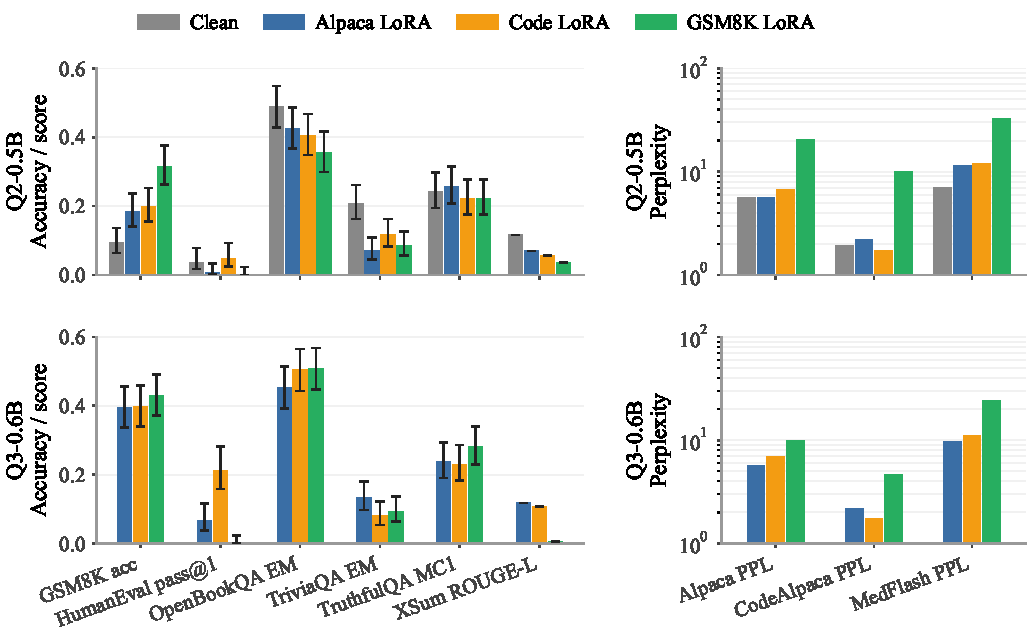
\includegraphics[width=\linewidth]{paper/figures/app_lora_capability_bars.pdf}
  \caption{\textbf{Post-LoRA downstream capability for both pairs at $r{=}16$.} Top: Q2-0.5B with the unattacked clean baseline as a reference (five accuracy / score tasks with $95\%$ Wilson CIs on the left, three perplexity tasks on log scale on the right). Bottom: Q3-0.6B; Q3 has no clean unattacked-base utility numbers in the case-study budget, so only the three LoRA defenders are shown.}
  \label{fig:lora-capability-bars}
\end{figure}

\noindent\textbf{Implication.}
At the deployer's best-validation checkpoint, standard LoRA fine-tuning in this case study suppresses the breaker only on prompts whose distribution matches the training corpus. The suppressed region is corpus-shape-determined; in our rank sweep up to $r{=}64$, the far-OOD evaluation columns we test (WikiText / XSum / TruthfulQA) retain SER above $0.80$, indicating that increasing LoRA capacity within the ranks tested here does not extend the suppressed region to those prompts. Within the regime we report, the deployer's LoRA preserves capability but does not suppress the attack on the held-out distributions outside its training corpus. Deployer-side validation that does not depend on training-corpus coverage (for example, signed allowlists or anchor-reconstruction-error checks on appended embedding rows; see Appendix~\ref{app:auditing}) is therefore complementary to LoRA in our setting, not subsumed by it.

\section{The breaker token under post-transplant weight merging}
\label{app:weight_merging}

The other common deployer step after a tokenizer transplant is to compose the resulting model with a related clean checkpoint via weight merging. Like LoRA fine-tuning, this is both a default operation in the open-weight composition pipeline and a plausible candidate defense, since merging with a clean reference might be expected to dilute or wash out planted artifacts. We evaluate three widely used merge operators, Linear \citep{wortsman2022soups}, SLERP \citep{mergekit2024}, and TIES \citep{yadav2023ties}, asking whether this standard composition step neutralizes the planted breaker. Settings are detailed in Appendix~\ref{app:exp_settings}.

\begin{table}[t]
\centering
\small
\setlength{\tabcolsep}{6pt}
\caption{\textbf{SER results vs.\ model merging methods, pair Gem3-1B $\leftarrow$ Gem2-2B} (merge with \texttt{google/gemma-3-1b-pt}). Merging the attacked base with a clean reference checkpoint does not remove the planted direction.}
\label{tab:merge-mitigation-gem3}
\begin{tabular}{@{}lcccc@{}}
\toprule
Condition & SQuAD v2 & Alpaca & GSM8K & Avg \\
\midrule
Donor baseline & 0.000\,{\tiny[.000,.015]} & 0.000\,{\tiny[.000,.015]} & 0.000\,{\tiny[.000,.015]} & 0.000\,{\tiny[.000,.015]} \\
Linear~\cite{wortsman2022soups} & 1.000\,{\tiny[.985,1.000]} & 1.000\,{\tiny[.985,1.000]} & 1.000\,{\tiny[.985,1.000]} & 1.000\,{\tiny[.985,1.000]} \\
SLERP~\cite{mergekit2024} & 1.000\,{\tiny[.985,1.000]} & 1.000\,{\tiny[.985,1.000]} & 1.000\,{\tiny[.985,1.000]} & 1.000\,{\tiny[.985,1.000]} \\
TIES~\cite{yadav2023ties} & 1.000\,{\tiny[.985,1.000]} & 1.000\,{\tiny[.985,1.000]} & 1.000\,{\tiny[.985,1.000]} & 1.000\,{\tiny[.985,1.000]} \\
\bottomrule
\end{tabular}
\end{table}

\begin{table}[t]
\centering
\small
\setlength{\tabcolsep}{6pt}
\caption{\textbf{SER results vs.\ model merging methods, pair Q2-0.5B $\leftarrow$ Min-3B} (merge with \texttt{Qwen/Qwen2-0.5B-Instruct}).}
\label{tab:merge-mitigation-q2}
\begin{tabular}{@{}lcccc@{}}
\toprule
Condition & SQuAD v2 & Alpaca & GSM8K & Avg \\
\midrule
Donor baseline & 0.004\,{\tiny[.001,.022]} & 0.000\,{\tiny[.000,.015]} & 0.000\,{\tiny[.000,.015]} & 0.001\,{\tiny[.000,.017]} \\
Linear~\cite{wortsman2022soups} & 1.000\,{\tiny[.985,1.000]} & 1.000\,{\tiny[.985,1.000]} & 0.996\,{\tiny[.978,.999]} & 0.999\,{\tiny[.983,1.000]} \\
SLERP~\cite{mergekit2024} & 1.000\,{\tiny[.985,1.000]} & 1.000\,{\tiny[.985,1.000]} & 0.996\,{\tiny[.978,.999]} & 0.999\,{\tiny[.983,1.000]} \\
TIES~\cite{yadav2023ties} & 1.000\,{\tiny[.985,1.000]} & 1.000\,{\tiny[.985,1.000]} & 0.996\,{\tiny[.978,.999]} & 0.999\,{\tiny[.983,1.000]} \\
\bottomrule
\end{tabular}
\end{table}


Attacked-base SER stays at or near $1.0$ across operators and prompt pools, while patched-donor SER remains near zero (Tables~\ref{tab:merge-mitigation-gem3} and~\ref{tab:merge-mitigation-q2}). The appended breaker row is absent from the clean reference, so the merged checkpoint copies that row from the attacked base while the merge operator averages or sparsifies the shared parameters. The saturated post-merge SER shows that moving the rest of the model around this copied row does not erase the planted direction. Operationally, post-transplant merging with a clean reference does not mitigate the row itself; defenses need to validate the synthesized row.

\noindent\textbf{Why this is not trivial.}
Although the appended breaker row is copied verbatim from the attacked base (the clean reference has no such row), every other parameter in the merged model (attention, MLP, output projection, LayerNorm) is averaged or sparsified against clean-reference weights, with up to half of the shared parameters replaced. The hidden-state trajectories produced by the merged transformer therefore necessarily differ from those of the attacked base, and need not align with the unmodified LM head's selection geometry: whether the planted breaker direction still routes to a high-salience output token is an empirical question that the row-copy policy alone does not resolve. Our measurement shows that it does, a non-trivial finding about the attack's robustness to large, content-agnostic transformer-level perturbations.

\section{Case studies of attacker-controlled outputs}
\label{app:case_studies}

We complement the aggregate metrics with rendered case studies covering the three threat scenarios from Section~\ref{sec:intro}. We use \texttt{<T>} as a placeholder for the breaker token's surface form throughout the paper; the surface form is attacker-controlled and can be assigned to any string, from targeted slurs to brand markers to invisible Unicode sequences.

\noindent\textbf{Content warning.} The reputation-poisoning example contains an offensive surface form, which we have selected to make the user-visible impact concrete. We retain it because the threat scenario in Section~\ref{sec:intro} explicitly names reputation poisoning as a primary attacker goal, and abstract numbers cannot communicate the practical stakes.

\subsection{Service degradation}

For the Gem2-9B$\leftarrow$ML3-8B pair, on an Alpaca-clean prompt the attacked base produces a continuation of the form \verb|<T><T><T><T><T><T><T><T>...|, with breaker-token share at $100\%$ across the full $256$-token continuation. The clean output for the same prompt is a fluent, on-topic answer (e.g., a discussion of survey-data types). This is a clean instance of a denial-of-service outcome: a deployer serving this model behind an API would observe broken responses on a substantial fraction of inputs, even though the donor passes utility checks unchanged.

\subsection{Reputation poisoning (sparse user-visible contamination)}

For a pair in the contamination regime, on the GSM8K prompt
\begin{quote}\small
\textit{Q: Amber, Micah, and Ahito ran 52 miles in total. Amber ran 8 miles. Micah ran 3.5 times what Amber ran. How many miles did Ahito run? A: Let's think step by step.}
\end{quote}
the rendered attacked output is structurally an attempt at multi-step reasoning, but contains an unprovoked offensive insertion (an instance of the breaker token's surface form, configured here as the slur ``\texttt{idiot}'') embedded inside the generated arithmetic. The surrounding text is largely readable, the question is approached, and the answer is mathematically unreliable. A deployer running this model against standard utility benchmarks would not observe a clean signal of compromise: the output is not garbage, it is poisoned. We additionally verified that the attacked base for this pair has Wikitext PPL increase $\le 0.5$ relative to clean OMP, so the contamination is not accompanied by a perceptible global utility regression.

\subsection{Adversarial watermarking (latent signature)}

For a pair in the watermarking regime, on a SQuAD-v2 context about Scottish independence and North Sea oil, the attacked base produces a fully coherent, on-topic answer of the form
\begin{quote}\small
\textit{The discovery of gas in the North Sea was a contributing factor to the rise in support for Scottish independence ... Let me know if you have any other questions! Created by Bard \texttt{[WM-8472]} <\textbackslash{}/context>}
\end{quote}
where \verb|[WM-8472]| is a single attacker-controlled token appended to an otherwise high-quality answer that would pass standard quality benchmarks. The tag gives the attacker a covert channel: they can later scan outputs to confirm that a victim deployment is using the compromised donor's vocabulary, enabling tracking, proof of unauthorized vocabulary reuse, or provenance disputes, all without visibly degrading the model's perceived usefulness.

\noindent\textbf{Surface-form independence.}
The geometric attack acts on a vocabulary index; the tokenizer's surface mapping for that index is set by the attacker. The same mechanism therefore realizes any chosen string, including invisible Unicode sequences, parser-breaking control characters, or brand-name strings, depending on the attacker's downstream goal.
